\documentclass[12pt, a4paper]{book}

% -------------------------------
% Compilar con XeLaTeX 
% -------------------------------


% -------------------------------
% Comandos comunes
% -------------------------------
\newcommand{\uclm}{Universidad de Castilla-La Mancha\,}
\newcommand{\dsi}{Departamento de Sistemas Informáticos\,}
\newcommand{\esii}{Escuela Superior de Ingeniería Informática de Albacete\,}
\newcommand{\iiia}{Instituto de Investigación en Informática de Albacete\,}


% -------------------------------
% Comandos específicos
% -------------------------------
\newcommand{\autor}{Emilio José Roldán Navarro\,}
\newcommand{\titulo}{Implatación de técnicas y herramientas de pentesting en el proceso de desarrollo de software\,}
\newcommand{\director}{Nombre del director\,}
\newcommand{\codirector}{Nombre del codirector\,}
\newcommand{\fecha}{Junio, 2021\,}
\newcommand{\espec}{Tecnología específica\,} 
\renewcommand{\chaptername}{Capitulo}






% -------------------------------
% Plantilla del TFG en la ESIIAB-UCLM. Versión 0.0 (Preliminar)
% 
% Compilar con XeLaTeX 
% -------------------------------
%\usepackage{fvextra,csquotes,xcolor,minted, graphicx, subcaption, url, multicol}
\usepackage{fvextra,csquotes,minted, graphicx, subcaption, url, multicol}
\usepackage[colorlinks=true, allcolors=blue]{hyperref}

%\usepackage[backend=biber,style=verbose-note]{biblatex}


% -------------------------------
% Idioma
% -------------------------------
\usepackage{polyglossia}
\setmainlanguage{spanish}

\usepackage[xindy,style=altlistgroup]{glossaries}
%\usepackage[toc]{glossaries}

% -------------------------------
% Fuente
% -------------------------------
% Cualquier tamaño de texto: {\fontsize{100pt}{120pt}\selectfont tutexto}
\usepackage{anyfontsize}
% Selección de fuentes.
\usepackage{fontspec}
% Espacio entre líneas
\usepackage{setspace}
% Fuentes especiales
\usepackage{textcomp,marvosym,pifont}
\usepackage[sfdefault,lf]{carlito}


% -------------------------------
% Otros paquetes de uso común
% -------------------------------
% Símbolos matemáticos
\usepackage{amsmath,amsfonts,amssymb}
% Gráficos
\usepackage{graphicx}
% Posición arbitraria de los gráficos
\usepackage[absolute,overlay]{textpos}
% Apéndices
\usepackage{appendix}


% -------------------------------
% Esquema de colores
% -------------------------------
% Paquete para la definición de colores
\usepackage[table]{xcolor}
% Esquema de colores
% -------------------------------
% Plantilla del TFG en la ESIIAB-UCLM. Versión 0.0 (Preliminar)
% 
% Compilar con XeLaTeX 
% -------------------------------

% -------------------------------
% Color del tema
% -------------------------------

% Color para los títulos, etc.
%\definecolor{tema}{RGB}{0,0,0}        % Negro 
%\definecolor{tema}{RGB}{182,0,52}     % LOGO UCLM
\definecolor{tema}{RGB}{0,69,134}      % Azul del esquema  
%\definecolor{tema}{RGB}{197,0,11}     % Rojo del esquema     

% Negritas con el color del tema
\newcommand{\bft}[1]{\textcolor{tema}{\bf #1}} 


% -------------------------------
% Esquema de colores
% -------------------------------
% Estos balores coinciden con colores de OpenOffice 
% Se pueden redefinir para que coincidan con las paletas de las 
% herramientas utilizadas para hacer las gráficas.
\definecolor{blanco}{RGB}{255,255,255} 
\definecolor{negro}{RGB}{0,0,0}
\definecolor{gris95}{gray}{.95}
\definecolor{gris75}{gray}{.75}
\definecolor{gris50}{gray}{.50}
\definecolor{gris25}{gray}{.25}
\definecolor{rojo}{RGB}{197,0,11}        % Gráfico 11
\definecolor{azul}{RGB}{0,69,134}        % Gráfico 1
\definecolor{verde}{RGB}{87,157,28}      % Gráfico 4
\definecolor{naranja}{RGB}{255, 149, 14} % Gráfico 10
\definecolor{mostaza}{RGB}{255, 211, 32} % Gráfico 3

% Negrita con color definido 
\newcommand{\bfa}[1]{\textcolor{azul}{\bf #1}} 
\newcommand{\bfr}[1]{\textcolor{rojo}{\bf #1}}
\newcommand{\bfn}[1]{\textcolor{naranja}{\bf #1}}
\newcommand{\bfv}[1]{\textcolor{verde}{\bf #1}}  
\newcommand{\bfm}[1]{\textcolor{mostaza}{\bf #1}} 






% -------------------------------
% Márgenes
% -------------------------------
% Márgenes de las páginas
\usepackage[
  inner	 =	3cm,   % Margen interior
  outer	 =	2.5cm, % Margen exterior
  top	 =	2.5cm, % Margen superior
  bottom =	2.5cm, % Margen inferior
  includeheadfoot, % Incluye cabecera y pie de página en los márgenes
]{geometry}
% Muestra una regla para comprobar el formato de las páginas (descomentar)
%\usepackage[type=upperleft,showframe,marklength=8mm]{fgruler} 


% -------------------------------
% Renombra tablas y bibliografía
% -------------------------------
\addto\captionsspanish{
	\renewcommand{\listtablename}{Índice de tablas} 
	\renewcommand{\tablename}{Tabla}
	\renewcommand{\bibname}{Referencia bibliográfica}
}


% -------------------------------
% Itemize y enumerate. Control de los espacios.
% -------------------------------
\usepackage{enumitem}
\setitemize{itemsep=0pt}
\setenumerate{itemsep=0pt}
\renewcommand{\labelitemi}{\tiny\bft{$\blacksquare$}}
\renewcommand{\labelitemii}{\bft{$\bullet$}}
\renewcommand{\labelitemiii}{\bft{-}}


% -------------------------------
% Enlaces y colores
% -------------------------------

%\hypersetup{
%    colorlinks,
%    citecolor=black,
%    filecolor=black,
%    linkcolor=black,
%    urlcolor=black
%}

% -------------------------------
% Gestión de elementos flotantes
% -------------------------------
% Para forzar a que las figuras aparezcan antes del fin de una sección.
%\usepackage[section]{placeins}

% Gestión de títulos de los elementos flotantes
\usepackage{caption}
% Subfiguras y títulos en subfiguras
\usepackage{subcaption}

% Títulos
\DeclareCaptionFont{tema}{\color{tema}} % Color
\captionsetup{labelfont={tema, bf}}     % Estilo
\captionsetup{font=normalsize}          % Tamaño
\captionsetup{width=.9\linewidth}       % Anchura del título
 % Distancia de la figura al texto.
\setlength{\intextsep}{1cm} 
\setlength{\textfloatsep}{1cm}         
       

% -------------------------------
% Utilidades para tablas
% -------------------------------
% Para fundir filas en tablas
\usepackage{multirow}
% Para definir columnas con ancho fijo y alineación
\usepackage{array,ragged2e}
\newcolumntype{L}[1]{>{\raggedright\let\newline\\\arraybackslash\hspace{0pt}}m{#1}}
\newcolumntype{C}[1]{>{\centering\let\newline\\\arraybackslash\hspace{0pt}}m{#1}}
\newcolumntype{R}[1]{>{\raggedleft\let\newline\\\arraybackslash\hspace{0pt}}m{#1}}


% -------------------------------
% Para tabular
% -------------------------------
\usepackage{tabto}


% -------------------------------
% Formato de títulos, capítulos, etc.
% -------------------------------
\usepackage{titlesec, titletoc}
% Parte
\titleformat{\part}[display]												   	   % Estilo
	{\Huge \centering \color{tema}}                                                % Formato
	{Parte \thepart }                                                              % Etiqueta
	{0.75ex}                                                                       % Separación
	{\bfseries\fontsize{25pt}{40pt}\selectfont}                                    % Entre etiqueta y título            
	[\thispagestyle{empty}]                                                        % Después

% Capítulo		
\titleformat{\chapter}[block]            			 			                    % Estilo  	
	{\vspace{0cm} \flushright \bfseries \LARGE \color{tema}}  	        			% Formato 
	{\thechapter.}                  			  									% Etiqueta
	{0.75ex}                                     									% Separación
	{}                                           									% Entre etiqueta y título
	[\vspace{0.1cm} \rule{0.5\textwidth}{1pt}\vspace*{1cm}\thispagestyle{plain}]    % Después      
  
% Sección
\titleformat{\section}
	{\vspace{5pt}  \Large \color{tema}}
	{\thesection .}
	{0.75ex}
	{}

% Subsección
\titleformat{\subsection}
	{\large \color{tema}}
	{\thesubsection .}
	{0.75ex}
	{}
 
% Subsubsección
\titleformat{\subsubsection}
	{\bf\color{tema}}
	{}
	{0.75ex}
	{}
	 
% Parte (TOC)
\titlecontents{part}[2pc]
  	{\vspace{20pt}\bfseries\filright\Large\color{tema}}
  	{\contentslabel{1.5pc}}{\hspace*{-1.5pc}}
  	{\vspace{5pt}}
  	{}
  
% Capítulo (TOC)
\titlecontents{chapter}[2pc]
  	{\vspace{10pt}\bfseries\large\filright}
  	{\contentslabel{1.5pc}}{\hspace*{-1.5pc}}
  	{\mdseries\titlerule*[0.5pc]{.}\bfseries\contentspage}

% Sección (TOC)
\titlecontents{section}[4pc]
  	{\vspace{5pt}\filright}
  	{\contentslabel{2pc}}{\hspace*{2pc}}
  	{\titlerule*[0.5pc]{.}\contentspage}
  	{\vspace{5pt}

% Subsección (TOC)
\titlecontents{subsection}[6pc]
  	{\vspace{2.5pt}\filright\small\em}
  	{\contentslabel{3pc}}{\hspace*{-3pc}}
  	{\titlerule*[0.5pc]{.}\contentspage} 
  	
  	
% -------------------------------
% Cabeceras y pie de página
% -------------------------------
\usepackage{fancyhdr}
\pagestyle{fancy}
\fancyhf{}

% Permite incluir la parte. Para ello crea \parttitle
\let\Oldpart\part
\newcommand{\parttitle}{}
\renewcommand{\part}[1]{\Oldpart{#1}\renewcommand{\parttitle}{#1}}

% Cabeceras y pies de página
\fancyhead[LE]{}
\fancyhead[RO]{\slshape \leftmark}
\fancyfoot[LE,RO]{\thepage}
\renewcommand{\footrulewidth}{1pt}
\renewcommand{\headrulewidth}{1pt}
\renewcommand{\chaptermark}[1]{\markboth{#1}{}} % Capítulo (Solo texto)
\renewcommand{\chaptermark}[1]{\markboth{\thechapter. #1}{}} % Capítulo (Número y texto)

% Formato plano para las páginas con títulos (solo incluye el pie de página)
\fancypagestyle{plain}{
\fancyhf{}
\fancyhead{}
\fancyfoot[LE,RO]{\thepage}
\renewcommand{\footrulewidth}{1pt}
\renewcommand{\headrulewidth}{0pt}
}

 
% -------------------------------
% Utilidades
% -------------------------------
% Marcas
\newcommand{\pcite}{\bfr{\large[?]}\,} % Cita pendiente: [?] en rojo y negrita.
\newcommand{\ps}{\bfr{\huge[--}\,} % Pricipio de un bloque en sucio
\newcommand{\fs}{\bfr{\huge--]}\,} % Fin de un bloque en sucio.

% Notas
\usepackage[textsize=tiny,spanish,shadow,textwidth=2cm]{todonotes}

% Para generar textos "random"
\usepackage{lipsum} 
 

% -------------------------------
% Algoritmos y código
% -------------------------------

% Se definen entornos específicos para algoritmos y código que permiten
% gestionar los títulos manera similar en ambos casos, y similar al resto
% de elementos flotantes.
\usepackage{newfloat}

\DeclareFloatingEnvironment[ % Algoritmos
  listname = {Índice de algoritmos},
  name = Algoritmo
]{algorithm}

\DeclareFloatingEnvironment[ % Fragmentos de código
  listname = {Índice de listados de código},
  name = Código
]{code}

% Define un estilo para el encabezado de algoritmos y código.
\DeclareCaptionFormat{algcode}{
% OPCIÓN 1 -> Línea debajo del título
\rule{\dimexpr\textwidth\relax}{0.4pt}\vspace{0cm}
#1#2#3
\vspace{-0.2cm}\rule{\dimexpr\textwidth\relax}{0.4pt} % 
% OPCIÓN 2 -> Sin línea debajo del título
%\rule{\dimexpr\textwidth\relax}{0.4pt}\vspace{0cm}
%#1#2#3
}
\captionsetup[algorithm]{format=algcode, width=\linewidth}
\captionsetup[code]{format=algcode, width=\linewidth}

% Opciones específicas para algoritmos.
\usepackage[noend]{algpseudocode}
% Tamaño de letra y separadores
\makeatletter
\renewcommand{\ALG@beginalgorithmic}{\small\hrule\vskip10pt}
\makeatother
% Variables y funciones
\newcommand{\va}[1]{{\it {#1}}}				
\newcommand{\fu}[1]{{\textsc{#1}}}          
% Palabras clave
\renewcommand{\algorithmicrepeat}{\bft{repetir}}
\renewcommand{\algorithmicuntil}{\bft{hasta}}
\renewcommand{\algorithmicend}{\bft{fin}}
\renewcommand{\algorithmicif}{\bft{si}}
\renewcommand{\algorithmicthen}{\bft{entonces}}
\renewcommand{\algorithmicelse}{\bft{si no}}
\newcommand{\algorithmicelsif}{\algorithmicelse\ \algorithmicif}
\newcommand{\algorithmicendif}{\algorithmicend\ \algorithmicif}
\renewcommand{\algorithmicfor}{\bft{para}}
\renewcommand{\algorithmicforall}{\bft{para cada}}
\renewcommand{\algorithmicwhile}{\bft{mientras}}
\renewcommand{\algorithmicdo}{\bft{hacer}}
\renewcommand{\algorithmicprocedure}{\bft{procedimiento}}
\renewcommand{\algorithmicreturn}{\bft{devolver}}
\renewcommand{\algorithmicfunction}{\bft{función}}
\renewcommand{\algorithmicloop}{\bft{iterar}}

% Opciones específicas para código.
\usepackage{listings}
% Aspecto de los listados de código (ejemplo)
% Los colores se han de cambiar y adaptar a los distintos lenguajes de programación.
\lstset{
    language=Python,
    keywordstyle=\bf\color{tema},  
	breaklines=true,    
	basicstyle={\small\ttfamily},
    tabsize=5,
    frame=t % Es importante no cambiar esta opción (es la línea superior) 
}

% -------------------------------
% Cacacteres pifont de uso común (con color)
% -------------------------------
\newcommand{\vmarkt}{\textcolor{tema}{\ding{52}} }  % Checked (V) Tema
\newcommand{\vmarkr}{\textcolor{rojo}{\ding{52}} }  % Checked (V) Rojo
\newcommand{\vmarka}{\textcolor{azul}{\ding{52}} }  % Checked (V) Azul

\newcommand{\xmarkt}{\textcolor{tema}{\ding{55}} }  % Checked (X) Tema
\newcommand{\xmarkr}{\textcolor{rojo}{\ding{55}} }  % Checked (X) Rojo
\newcommand{\xmarka}{\textcolor{azul}{\ding{55}} }  % Checked (X) Azul

\newcommand{\lmarkt}{\textcolor{tema}{\ding{46}} }  % Lápiz Tema
\newcommand{\lmarkr}{\textcolor{rojo}{\ding{46}} }  % Lápiz Rojo
\newcommand{\lmarka}{\textcolor{azul}{\ding{46}} }  % Lápiz Azul

\newcommand{\hmarkt}{\textcolor{tema}{\ding{43}} }  % Mano Tema
\newcommand{\hmarkr}{\textcolor{rojo}{\ding{43}} }  % Mano Roja 
\newcommand{\hmarka}{\textcolor{azul}{\ding{43}} }  % Mano Azula 

\newcommand{\fmarkt}{\textcolor{tema}{\ding{220}} }  % Flechza Tema
\newcommand{\fmarkr}{\textcolor{rojo}{\ding{220}} }  % Flecha Roja 
\newcommand{\fmarka}{\textcolor{azul}{\ding{220}} }  % Flecha Azul
% Generate the glossary
\makeglossaries
\loadglsentries{glosario}

\begin{document}
% -------------------------------
% Portada y título
% -------------------------------
% -------------------------------
% Plantilla del TFG en la ESIIAB-UCLM. Versión 0.0 (Preliminar)
% 
% Compilar con XeLaTeX 
% -------------------------------
\pagestyle{empty}
\begin{titlepage}\null



\begin{textblock*}{\paperwidth}(0cm,3cm)
\begin{center}

\includegraphics[width=4cm]{figs/logoconciti.png}
\end{center}
\end{textblock*}


\begin{textblock*}{\paperwidth}(0cm,8cm) 
\begin{center}\doublespacing
{\fontsize{16pt}{2pt}\selectfont Universidad de Castilla-La Mancha}

{\fontsize{16pt}{2pt}\selectfont Escuela Superior de Ingeniería Informática}
\end{center}
\end{textblock*}


\begin{textblock*}{\paperwidth}(0cm,12cm) 
\begin{center}\doublespacing 
{\bf\fontsize{18pt}{4pt}\selectfont Trabajo Fin de Grado}

{\fontsize{18pt}{4pt}\selectfont Grado en Ingeniería Informática}

{\fontsize{16pt}{4pt}\selectfont \espec}
\end{center}
\end{textblock*}


% El título ocupa el 80% de la página. Puede adaptarse 
% a la longitud del texto
\begin{textblock*}{0.8\paperwidth}(0.1\paperwidth,17.5cm) 
\begin{center}\doublespacing % onehalfspace
{\bf\fontsize{20pt}{4pt}\selectfont \titulo}

\vskip1cm
{\it \fontsize{18pt}{4pt}\selectfont \autor}
\end{center}
\end{textblock*}


\begin{textblock*}{\paperwidth}(0cm,25.5cm) 
\begin{center}
{\fontsize{14pt}{4pt}\selectfont \fecha}
\end{center}
\end{textblock*}
\end{titlepage}
\setmainfont{Carlito}
% -------------------------------
% Preámbulo
% -------------------------------
\frontmatter 
% -------------------------------
% Plantilla del TFG en la ESIIAB-UCLM. Versión 0.0 (Preliminar)
%
% Luis de la Ossa
% 
% Compilar con XeLaTeX 
% -------------------------------


% -------------------------------
% Segunda portada
% -------------------------------
\cleardoublepage
\setcounter{page}{1} \null

\begin{textblock*}{3cm}(3cm,2cm) 
\begin{flushleft}

\includegraphics[height=2cm]{figs/logouclm.png}
\end{flushleft}
\end{textblock*}


\begin{textblock*}{2.5cm}(15.95cm,2.45cm) 
\begin{flushright}

\includegraphics[height=1.4cm]{figs/euroinf.jpg}
\end{flushright}
\end{textblock*}

\begin{textblock*}{2cm}(14cm,2cm)  % Corrige la posición porque la imagen tiene margen
\begin{flushright}

\includegraphics[height=2cm]{figs/logoesii.png}
\end{flushright}
\end{textblock*}



\begin{textblock*}{\textwidth}(3cm,8cm) 
\begin{center}\doublespacing 
{\fontsize{18pt}{4pt}\selectfont \bft{TRABAJO FIN DE GRADO}}

\medskip
{\fontsize{18pt}{4pt}\selectfont Grado en Ingeniería Informática}

\medskip
{\fontsize{16pt}{4pt}\selectfont \espec}
\end{center}
\end{textblock*}


\begin{textblock*}{\textwidth}(3cm,14cm) 
\begin{center}\setstretch{2}
{\fontsize{22pt}{4pt}\selectfont \bft{\titulo}}
\end{center}
\end{textblock*}


\begin{textblock*}{\textwidth}(3cm,20.5cm) 
\begin{flushleft}\doublespacing
{\fontsize{14pt}{4pt}\selectfont \bft{Autor:} \autor}

{\fontsize{14pt}{4pt}\selectfont \bft{Tutor:} \director}

%{\fontsize{14pt}{4pt}\selectfont \bft{Co-Tutor:} \codirector}
\end{flushleft}
\end{textblock*}


\begin{textblock*}{\linewidth}(3cm,25cm) 
\begin{flushright}
{\fontsize{14pt}{4pt}\selectfont \fecha}
\end{flushright}
\end{textblock*}


% -------------------------------
% Dedicatoria
% -------------------------------
\cleardoublepage
\thispagestyle{empty}

\vspace*{9cm}  
\begin{flushright} \em 
Aquí va la dedicatoria que cada cual \\ 
quiera escribir. El ancho se controla \\ 
manualmente
\end{flushright}


% -------------------------------
% Declaración de autoría
% -------------------------------
\cleardoublepage
\thispagestyle{plain}
\begin{center}
\Large{\bft{Declaración de autoría}}
\end{center}
\vskip1cm

Yo, \quad \ldots \quad, con DNI \quad \ldots \quad, declaro que soy el único autor del trabajo fin de grado titulado ``\quad \ldots \quad'', que el citado trabajo no infringe las leyes en vigor sobre propiedad intelectual, y que todo el material no original contenido en dicho trabajo está apropiadamente atribuido a sus legítimos autores.

\vspace*{2cm}
\begin{center}
Albacete, a \quad \ldots \quad de \quad \ldots \quad de 20 \ldots

\vskip3cm

Fdo.: \autor
\end{center}


% -------------------------------
% Resumen
% -------------------------------
\cleardoublepage
\thispagestyle{plain}
\begin{center}
\Large{\bft{Resumen}}
\end{center}
\vskip1cm

\lipsum[1]

% -------------------------------
% Agradecimientos
% -------------------------------
\cleardoublepage
\thispagestyle{plain}
\begin{center}
\Large{\bft{Agradecimientos}}
\end{center}
\vskip1cm

\lipsum[1]

% -------------------------------
% Índices y tablas
% -------------------------------
\tableofcontents	% Índice
\listoffigures		% Índice de figuras
\listoftables		% Índice de tablas
\listofalgorithms   % Índice de algoritmos (comentar si no los hay)
\listofcodes	    % Índice de códigos (comentar si no los hay)
\cleardoublepage

% -------------------------------
% Documento
% -------------------------------
\mainmatter
% Estilo de página
\pagestyle{fancy}

\chapter{Introducción.}
\chapter{Introducción.}
\section{motivación y objetivos}

  El motivo principal que me ha llevado a realizar este proyecto es relatar como realizar un proceso 
de pentesting resaltando dos herramientas que a día de hoy hay muchos pentester que no suelen utilizar
como son los análisis de código, sobre todo la parte estática, así como la integración de dichas 
pruebas en el ciclo de desarrollo Software.

\clearpage

\chapter{Análisis del estado del arte}
\input{chapters/02_Análisis del estado del arte.tex} 
 
\chapter{Diseño solución técnica.}

\input{./chapters/031_MétodologiaPruebas.tex}

\section{Infraestructura de pruebas} 
Como entorno de pruebas para la ejecución de los análisis de código; haremos uso de una máquina física y de un contenedor 
de Docker con la siguientes características y herramientas instaladas en cada una de ellas:

\begin{table}[!htb]
    \begin{center}
      \begin{tabular}{c| c |c}
      \hline 
        \rowcolor{tema!10}
        \bft{Características} & \bft{Máquina física} & \bft{Contenedor}\\
        \hline
        Sistema Operativo & Windows 10 Pro & Debian GNU/Linux 10 (buster)\\  \hline
        \multirow{3}{4em}{Herramientas} & OWASP Zap 2.10 & SonarQube 8.2 \\
        & Dependency-check & PostGresSQL 13.3 \\ 
        & SonarScaner 4.6.2 &  \\ \hline
      \end{tabular}
      \caption{Infraestructura de pruebas}
      \label{tab:InfraestructuraPruebas}
    \end{center}
  \end{table}

Para levantar el contenedor podemos hacer uso de dockercompose incluido en la carpeta \textbf{"entornoPrueba"} dentro de 
las \href{https://github.com/M0l1n3ta/PFG/tree/master}{fuentes de proyecto}

Para levantar el entorno ejecutamos:\\

\begin{verbatim}
    docker-compose up
\end{verbatim}

\begin{figure}[!htb]
    \centering
    \captionsetup{width=1\linewidth}    
    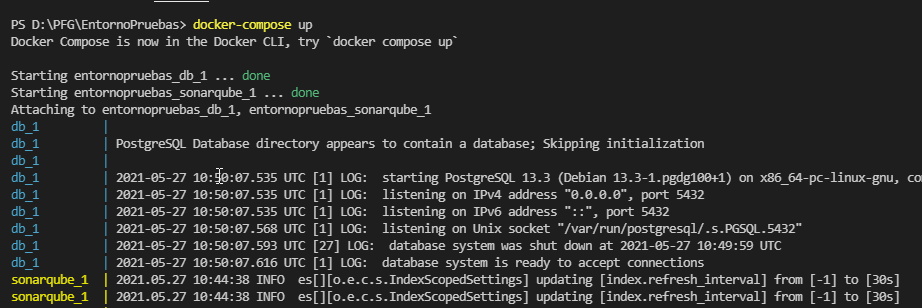
\includegraphics[width=\linewidth]{./imagenes/04_DockerCompose_UP.png}
    \caption{Docker compose up}  
\end{figure}

\clearpage
\newpage
Una vez que se veamos las siguientes líneas en el log:\\
\begin{figure}[!htb] 
    \captionsetup{width=1\linewidth}   
    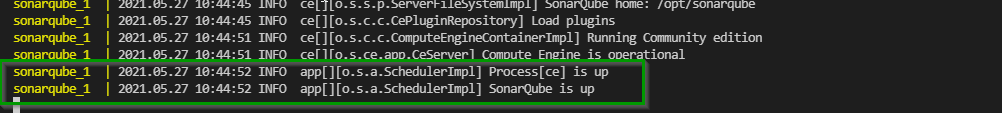
\includegraphics[width=\linewidth]{./imagenes/05_SonarQubeServerRunning.png}
    \caption{SonarQube server running}  
\end{figure}

Podremos acceder a la página de SonarQube en 
la url \href{http://localhost:9000}{http://localhost:9000}\\
\begin{figure}[!htb] 
    \captionsetup{width=1\linewidth}   
    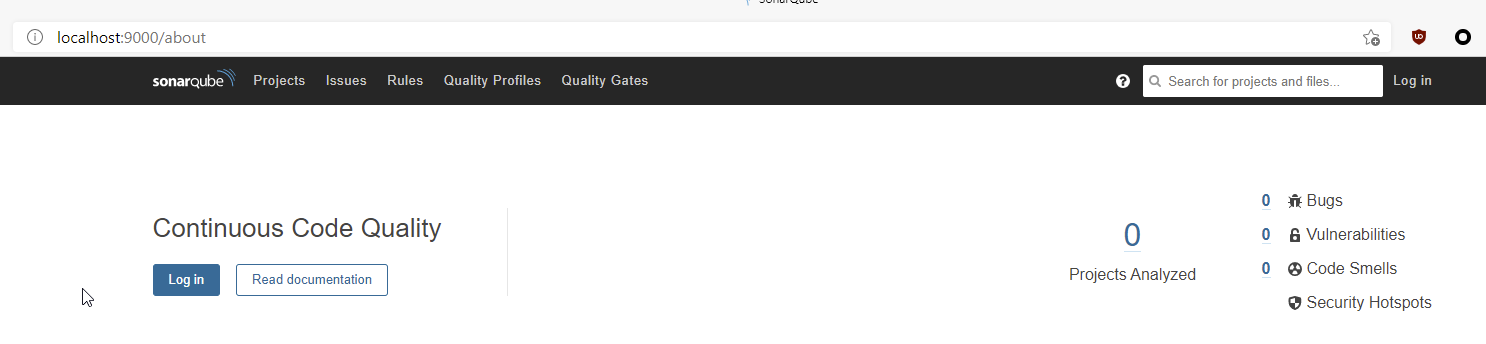
\includegraphics[width=\linewidth]{./imagenes/06_SonarQubeServer_Webpage.png}
    \caption{SonarQube portal}  
    \label{fig:21}
\end{figure}

\clearpage
\newpage
El fichero del docker compose \ref{alg:dockercompose} muestra los componentes de a aquitectura utilizados:

\begin{listing}
    \centering
    \inputminted{yaml}{./EntornoPruebas/SonarQube_8.2/docker-compose.yml}
    \caption{Docker Compose}
    \label{alg:dockercompose}
\end{listing}

\clearpage

\chapter{Ejecución casos de prueba.}
\section{Aplicación en desarrollo de aplicaciones Web} 

Como aplicaciones para los casos de prueba haremos uso de las siguientes aplicaciones:

\begin{table}
    \begin{center}
      \caption{Parámetros línea comandos dependency-check}
      \label{tab:tabla 2}
      \begin{tabular}{c|c}
        \textbf{Aplicación} & \textbf{Tecnologías utilizadas}\\
        \hline
        \href{https://dvwa.co.uk/}{Damn Vulnerable Web application (dwva)} & PHP\\ 
        \href{https://github.com/bkimminich/juice-shop}{Juice Shop} & JavaScript, Angular, Node.js\\
        \href{https://github.com/WebGoat/WebGoat}{WebGoat} &  Java, Spring Boot\\
        \href{https://github.com/tobyash86/WebGoat.NET}{WebGoat.Net} & .Net Core     
      \end{tabular}
    \end{center}
  \end{table}

\subsubsection{Damn Vulnerable Web application (DVWA)}

Siguiendo las tareas del \href{https://github.com/M0l1n3ta/PFG/blob/master/Reportes/DVWA/PPR DVWA - Plan Pruebas de Seguridad.docx}{documento de plan pruebas}
para este proyecto, realizamos las tareas que se detallan a continuación.

Para este proyecto no se realizará análisis de dependencias puesto que el proyecto no hace uso del componente de PHP 
necesario para realizar este tipo de análisis en proyectos PHP (\href{https://getcomposer.org/}{Composer})

La ejecución del análisis estático de código lo realizaremos a través de un
\href{https://github.com/M0l1n3ta/PFG/blob/master/Scripts/STAT/RunSonarScaner_DWVA.ps1}{script}, con el cual obtenemos 
el siguiente resultado:

\begin{figure}[h!]  
    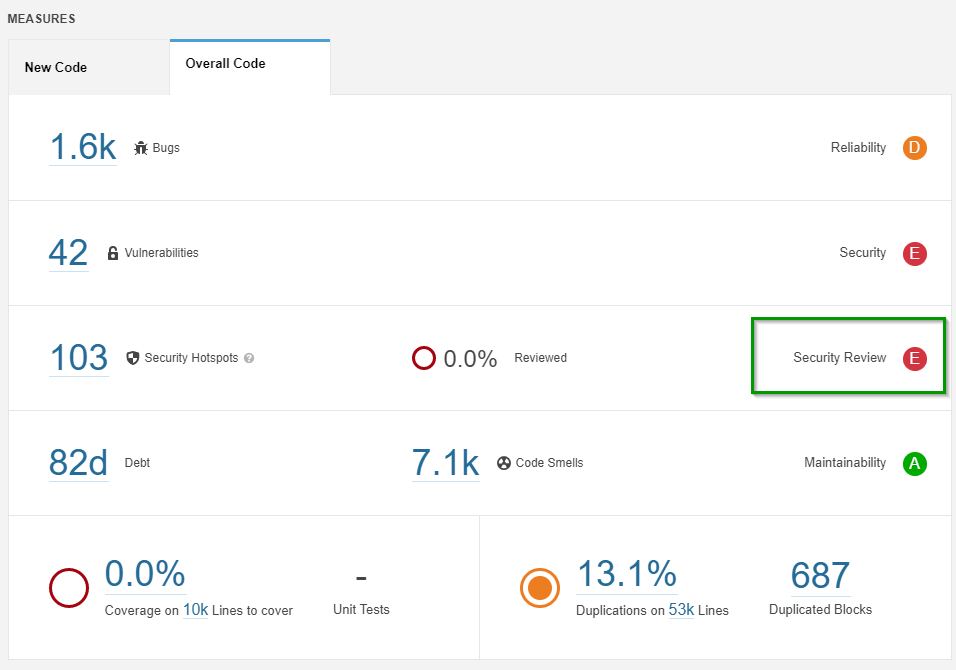
\includegraphics[width=\linewidth]{./imagenes/07_AnalisisEstatico__DVWA.png}
    \caption{Resultado análisis estatico código DVWA}  
    \label{fig:7}
\end{figure}
Como era de esperar obtiene el peor resultado posible en la medida de seguridad \textbf{“E”}

\subsubsection{Juice Shop}
Siguiendo las tareas del documento de plan pruebas para este proyecto, realizamos las tareas que se detallan a continuación.
La ejecución del análisis estático de código, así como el análisis de dependencias, lo realizaremos a través de un 
\href{https://github.com/M0l1n3ta/PFG/blob/master/Scripts/STAT/RunSonarScaner_JuiceShop.ps1}{script}, con el cual obtenemos 
el siguiente resultado:

\begin{figure}[h!]  
    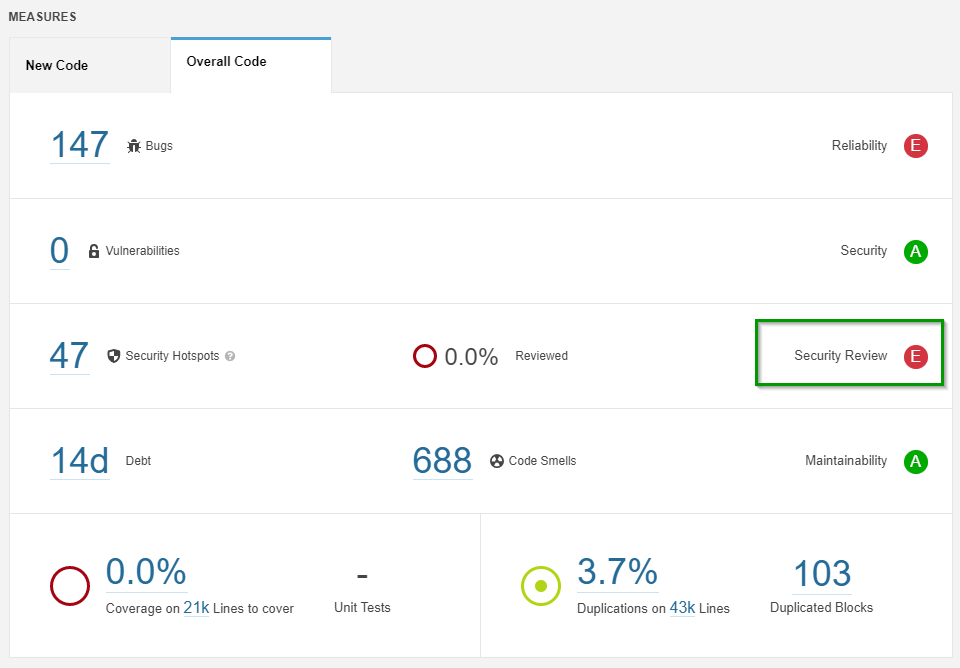
\includegraphics[width=\linewidth]{./imagenes/08_AnalisisEstatico_JuiceShop.png}
    \caption{Resultado análisis estatico código Juice Shop}  
    \label{fig:8}
\end{figure}
Como era de esperar obtiene el peor resultado posible en la medida de seguridad \textbf{“E”}

\subsubsection{WebGoat}
Siguiendo las tareas del documento de plan pruebas para este proyecto, realizamos las tareas que se detallan a continuación.

Para ejecutar el análisis de dependencias desde Maven, debemos añadir la siguiente configuración del plugin de Dependency-Check:

\begin{listing}[ht]
    \inputminted{xml}{./Ficheros/ConfiguracionPlugin_Maven.xml}
    \caption{Example from external file}
    \label{listing:4}
\end{listing}
A parte de la configuración anterior debemos añadir las siguientes propiedades:
\begin{listing}[ht]
    \inputminted{xml}{./Ficheros/ConfigPropertiesPlugin_maven.xml}
    \caption{Example from external file}
    \label{listing:4}
\end{listing}
Para ejecutar el escáner
\begin{verbatim}
    mvn dependency-check:check
\end{verbatim}

La ejecución del análisis estático de código, así como el análisis de dependencias, lo realizaremos a través de un 
\href{https://github.com/M0l1n3ta/PFG/blob/master/Scripts/STAT/RunSonarScaner_WebGoat.ps1}{script}, con el cual
obtenemos el siguiente resultado:
\begin{figure}[h!]  
    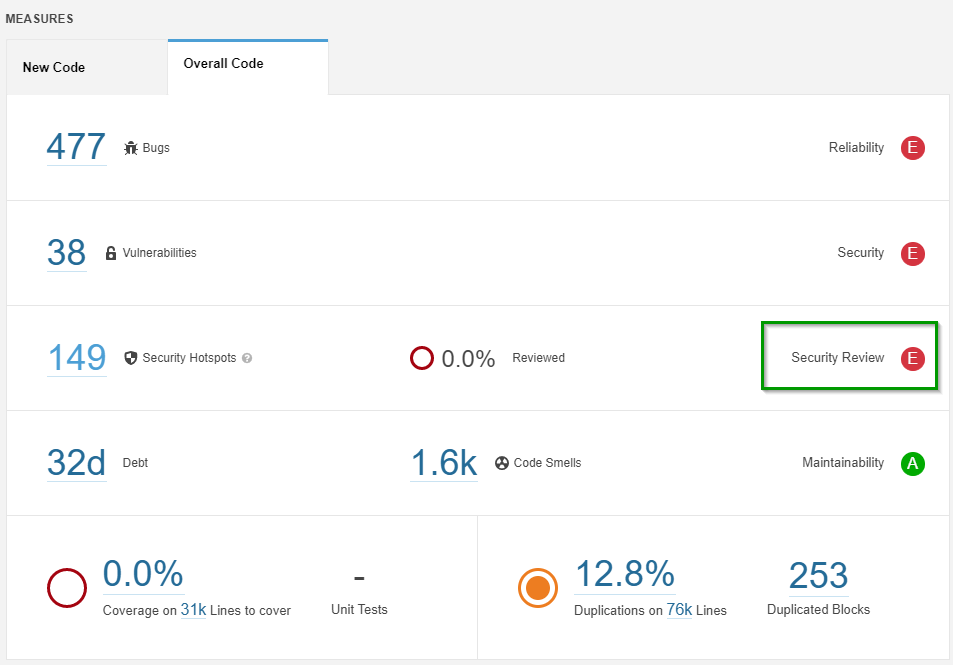
\includegraphics[width=\linewidth]{./imagenes/09_AnalisisEstatico_WebGoat.png}
    \caption{Resultado análisis estatico código WebGoat}  
    \label{fig:9}
\end{figure}
Como era de esperar obtiene el peor resultado posible en la medida de seguridad \textbf{“E”}

\subsubsection{WebGoat.Net}
Siguiendo las tareas del documento de plan pruebas para este proyecto, realizamos las tareas que se detallan a continuación.

La ejecución del análisis estático de código, así como el análisis de dependencias, lo realizaremos a través de un 
\href{https://github.com/M0l1n3ta/PFG/blob/master/Scripts/STAT/RunSonarScaner_WebGoat.NET.ps1}{script}, con el cual obtenemos
el siguiente resultado:
\begin{figure}[h!]  
    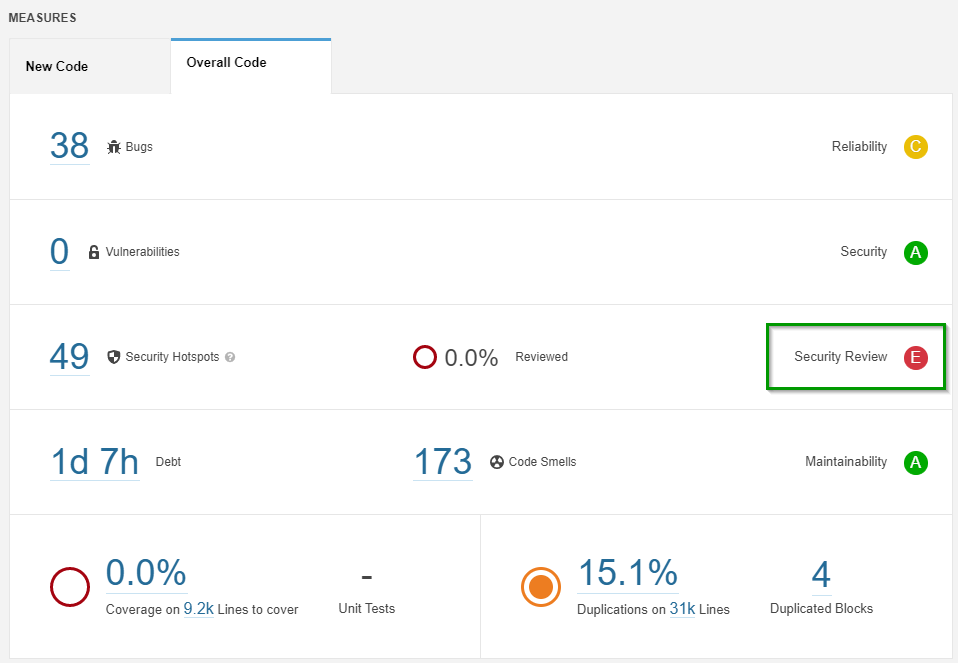
\includegraphics[width=\linewidth]{./imagenes/10_AnalisisEstatico_WebGoat.Net.png}
    \caption{Resultado análisis estatico código WebGoat}  
    \label{fig:9}
\end{figure}
Como era de esperar obtiene el peor resultado posible en la medida de seguridad \textbf{“E”}

\section{Aplicación en desarrollo de Servicios Web} 





% -------------------------------
% Apéndices
% -------------------------------
\appendix
\chapter{Anexo 1}
\lipsum[1-2]

\cleardoublepage
\thispagestyle{empty}

%\addbibresource{bibliografia.bib} 
%\printbibliography[title=Bibliografia]
% -------------------------------
% Bibliografía
% -------------------------------
\bibliographystyle{apalike}
\bibliography{bib/ref} 
\addcontentsline{toc}{chapter}{Referencia bibliográfica} % Añade a la tabla de contenidos

%Print the glossary
\printglossaries

\end{document}